\subsection{PRELIMINARY RESULTS}

Lemma 1. The set of hyperplanes \(\mathfrak{H}\) is locally finite.

Indeed, let K be a compact subset of E. If a hyperplane \(H \in H\) meets K, the set \(s_{\mathrm{H}}(\mathrm{K})\) also meets K, since every point of \(K \cap H\) is fixed by \(s_{H}\) . The set of \(H \in H\) meeting K is thus finite by (D'2).

We can thus apply to E and H the definitions and results of §1. We shall call the chambers, facets, walls, etc. defined in E by H simply the chambers, facets, walls, etc. relative to W. Any displacement \(w \in W\) permutes the chambers, facets, walls, etc.

Lemma 2. Let C be a chamber.

\begin{enumerate}
\def\labelenumi{(\roman{enumi})}
\item
  For any \(x \in \mathrm{E}\) , there exists an element \(w \in \mathrm{W}\) such that \(w(x) \in \overline{\mathrm{C}}\) .
\item
  For any chamber \(\mathrm{C}'\) , there is an element \(w \in \mathrm{W}\) such that \(w(\mathrm{C}') = \mathrm{C}\) .
\item
  The group W is generated by the set of orthogonal reflections with respect to the walls of C.
\end{enumerate}

Let M be the set of walls of C and let \(W_{M}\) be the subgroup of W generated by the reflections with respect to the walls of C.

\begin{enumerate}
\def\labelenumi{(\roman{enumi})}
\tightlist
\item
  Let \(x \in E\) and let \(J\) be the orbit of \(x\) under the group \(W_{\mathfrak{M}}\) . It suffices to prove that \(J\) meets \(\overline{C}\) .
\end{enumerate}

Let \(a\) be a point of \(C\) ; there is a closed ball \(B\) with centre \(a\) meeting \(J\) ; since \(B\) is compact, property (D'2) of no. 1 shows that \(B \cap J\) is finite. Hence, there exists a point \(y\) of \(J\) such that

\[
d (a, y) \leqslant d (a, y ^ {\prime}) \quad \text { for   all } y ^ {\prime} \text { in } J.\tag{1}
\]

We shall prove that \(y \in \overline{\mathbb{C}}\) . For this, it suffices to show that if \(H\) is a wall of \(C\) then \(y \in \overline{\mathrm{D}_{\mathrm{H}}(C)}\) (cf.~§ 1, no. 4, Prop. 9). Since \(s_H \in W_{\mathfrak{M}}\) , we have \(s_H(y) \in J\) and so (fig.~1)

\[
d (a, y) ^ {2} \leqslant d (a, s _ {\mathrm{H}} (y)) ^ {2}\tag{2}
\]

by (1). There exist \(b \in \mathbf{H}\) and two vectors \(t\) and \(u\) such that \(a = b + t\) and \(y = b + u\) , the vector \(u\) being orthogonal to \(\mathbf{H}\) ; then \(s_{\mathrm{H}}(y) = b - u\) , and (2)

is equivalent to \((t - u|t - u) \leqslant (t + u|t + u)\) , or to \((t|u) \geqslant 0\) . This inequality implies that \(y \in \overline{\mathrm{D}_{\mathrm{H}}(\mathrm{C})}\) .

\pandocbounded{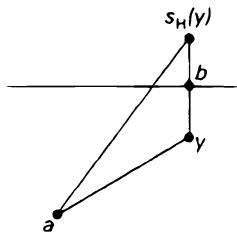
\includegraphics[keepaspectratio]{images/part001_5f5a2798.jpg}}\\
Fig. 1

\begin{enumerate}
\def\labelenumi{(\roman{enumi})}
\setcounter{enumi}{1}
\item
  Let \(\mathbf{C}'\) be a chamber and \(a' \in \mathbf{C}'\) . By what we have proved, there exists \(w \in \mathrm{W}_{\mathfrak{M}}\) such that \(w^{-1}(a') \in \overline{\mathbf{C}}\) ; hence, the chamber \(\mathbf{C}'\) meets \(\overline{w(\mathbf{C})}\) ; since \(\overline{w(\mathbf{C})}\) is the union of \(w(\mathbf{C})\) and facets with empty interior (§ 1, no. 2, Prop. 3), we have \(\mathbf{C}' = w(\mathbf{C})\) .
\item
  We have to prove that \(W = W_{\mathfrak{M}}\) and for this it suffices to prove that \(s_{H'} \in W_{\mathfrak{M}}\) for all \(H' \in \mathfrak{H}\) . Now \(H'\) is a wall of at least one chamber \(C'\) (§1, no. 4, Prop. 8); we have seen that there exists \(w \in W_{\mathfrak{M}}\) such that \(C' = w(C)\) ; consequently, there exists a wall \(H\) of \(C\) such that \(H' = w(H)\) , hence \(s_{H'} = w.s_H.w^{-1} \in W_{\mathfrak{M}}\) .
\end{enumerate}

